\section{Introducción}

% Sondas de red
\begin{frame}{Sondas de red}
  \begin{itemize}
    \item Dispositivos capaces de capturar y/o inyectar tráfico de red
    \item Principales usos
    \begin{itemize}
      \item Análisis de las trazas capturadas por la sonda
      \item Realización de pruebas sobre redes, plataformas y aplicaciones
    \end{itemize}
    \item Diferentes tipos sobre ordenadores convencionales
    \begin{itemize}
      \item Tarjetas Ethernet estándar
      \item Tarjetas a medida basadas en FPGAs
    \end{itemize}
  \end{itemize}
\end{frame}

% Sonda utilizada
\begin{frame}{Sonda utilizada - NetFPGA 10G}
  \begin{itemize}
    \item Sonda a medida basada en FPGA
    \begin{itemize}
      \item Modelo Xilinx Virtex-5
      \item Cuatro interfaces SFP+ de hasta 10Gbps
      \item Conectada por PCI Express
    \end{itemize}
    \item Permite capturar y reproducir tráfico de red
    \item Rendimiento máximo de 10 Gbps por linea (cuatro en total)
    \item Gestionada por línea de comandos
  \end{itemize}
  \begin{figure}
    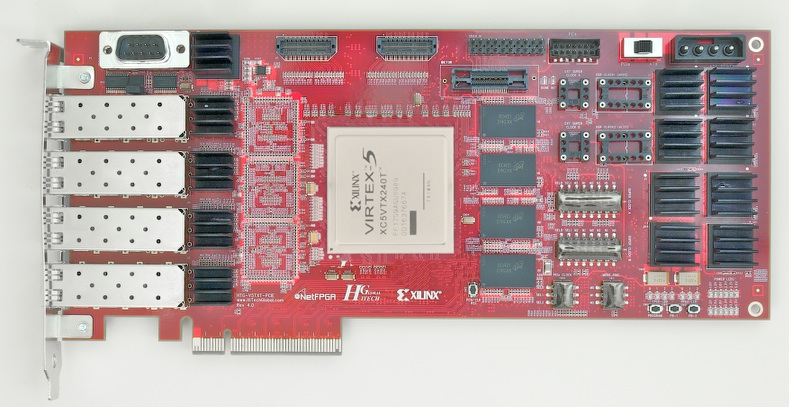
\includegraphics[width=0.6\linewidth]{NetFPGA10G}
  \end{figure}
\end{frame}
